\documentclass[a4paper, 12pt]{article}

\usepackage[T2A]{fontenc}
\usepackage[utf8]{inputenc}
\usepackage[english,russian]{babel}
\usepackage[left=15mm, top=20mm, right=15mm, bottom=20mm, nohead, nofoot]{geometry}

\usepackage{hyperref}

\usepackage{wrapfig}
\usepackage{afterpage}
\usepackage{amsmath, amsfonts, amssymb, amsthm, mathtools}
\author{}
\title{}
\date{}
%%%%%%%%%%%%%%%%%%%%%%%%%%%%%%%%%%%%%%%%%%%%%%%%%%%%%%%%%%%%%%%%%%%%%%%%%
\usepackage{fancyhdr}
\usepackage{lastpage}
\usepackage{graphicx, wrapfig, subcaption, setspace, booktabs}
\usepackage[T1]{fontenc}
\usepackage[font=small, labelfont=bf]{caption}
\usepackage[protrusion=true, expansion=true]{microtype}
\usepackage[english]{babel}
\usepackage{sectsty}
\usepackage{url, lipsum}
\newcommand{\HRule}[1]{\rule{\linewidth}{#1}}
\onehalfspacing
\setcounter{tocdepth}{5}
\setcounter{secnumdepth}{5}

\usepackage{graphicx}
\graphicspath{{pictures/}}
\DeclareGraphicsExtensions{.pdf,.png,.jpg}
\usepackage{multirow}

\usepackage[autoplay, loop, nomouse, controls]{ animate}
\usepackage[autoplay, repeat]{ movie 15}
%%%%%%%%%%%%%%%%%%%%%%%%%%%%%%%%%%%%%%%%%%%%%%%%%%%%%%%%%%%%%%%%%%%%%%%%%


\begin{document}

\title{ \normalsize \textsc{ОТЧЕТ}
		\\ [4.0cm]
		\HRule{0.5pt} \\ [0.3cm]
		\LARGE \textbf{{ПЕРВОЕ ЗАДАНИЕ}}
		\HRule{0.5pt} \\ [0.1cm]
		\normalsize  \vspace*{20\baselineskip}}

\date{}

\author{
		Маллаев Руслан, Б02-005 \\
ЛФИ, 2022\\ }

\maketitle
\thispagestyle{empty}
\newpage

\part{Установление распределения Максвелла}

\begin{center}
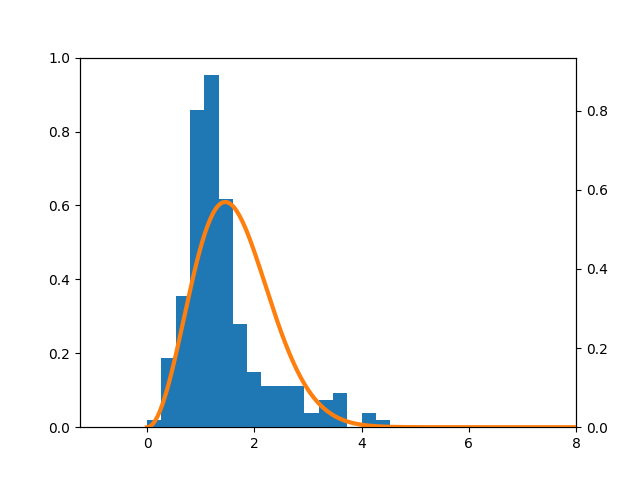
\includegraphics[scale=0.8]{40}
\end{center}
\[\textit{40-ой шаг}\]
\begin{center}
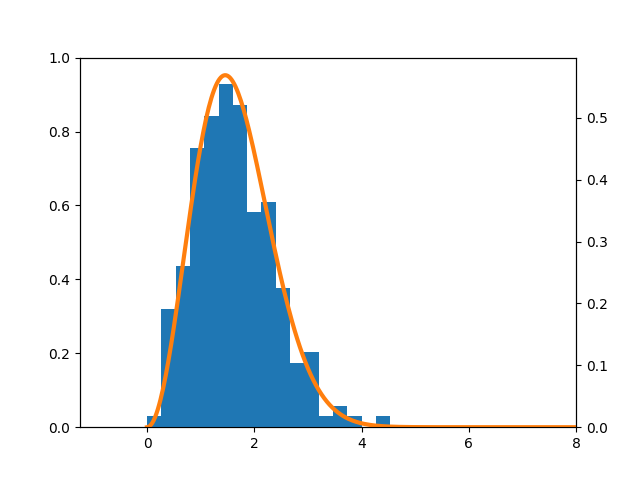
\includegraphics[scale=0.8]{660}
\end{center}
\[\textit{660-ой шаг}\]\\\\
В модели 216 частиц с dt = 0.001 с изначально случайно распределенными скоростями. Распределение начинает устанавливаться уже на $\sim$ 300 шаге, но окончательно вписывается в теоретически построенное распределение на $\sim$ 650 шаге.\\
Теоретическая кривая соответствует распределению Максвелла по модулю скорости соответствующему установившейся температуре T $\approx$ 1, но с подобранным масштабирующим коэффициентом (по вертикали).

\part{Время динамической памяти}

\begin{minipage}{0.47\textwidth}
\begin{center}
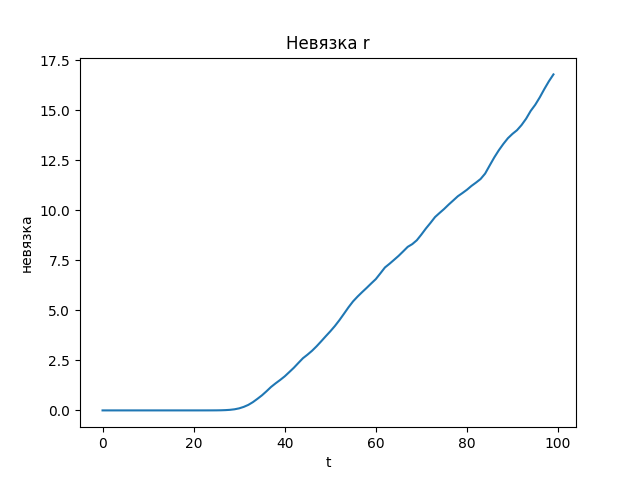
\includegraphics[scale=0.6]{r_div2}
\end{center}
\end{minipage}
\begin{minipage}{0.47\textwidth}
\begin{center}
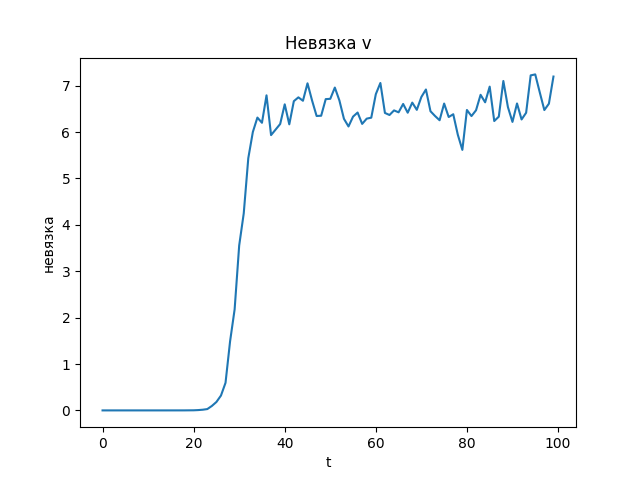
\includegraphics[scale=0.6]{v_div2}
\end{center}
\end{minipage}
\[\textit{Невязки при ratio = 2}\]
\begin{minipage}{0.47\textwidth}
\begin{center}
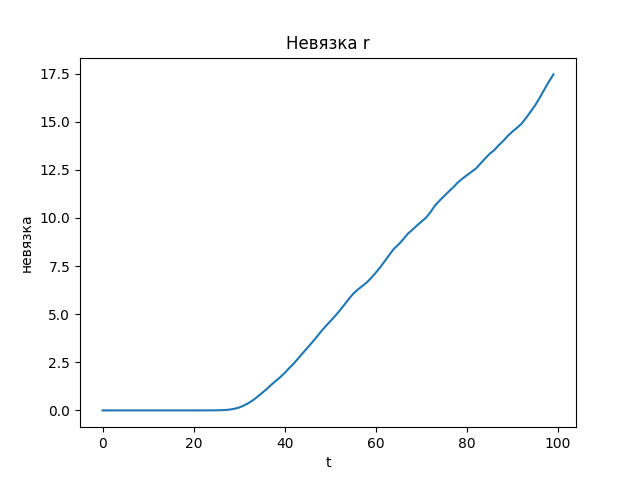
\includegraphics[scale=0.6]{r_div5}
\end{center}
\end{minipage}
\begin{minipage}{0.47\textwidth}
\begin{center}
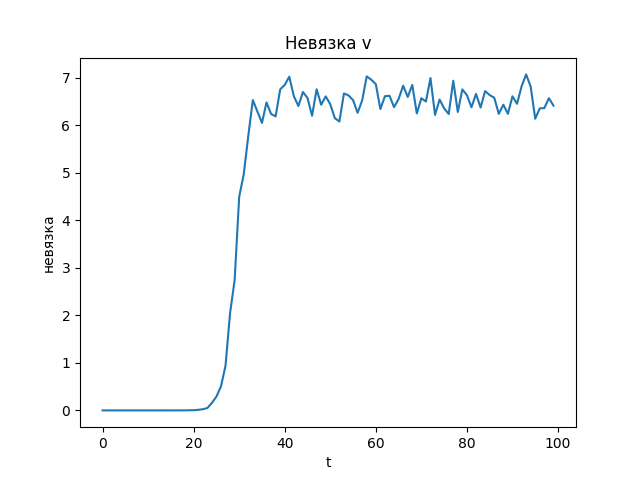
\includegraphics[scale=0.6]{v_div5}
\end{center}
\end{minipage}
\[\textit{Невязки при ratio = 5}\]
\begin{minipage}{0.47\textwidth}
\begin{center}
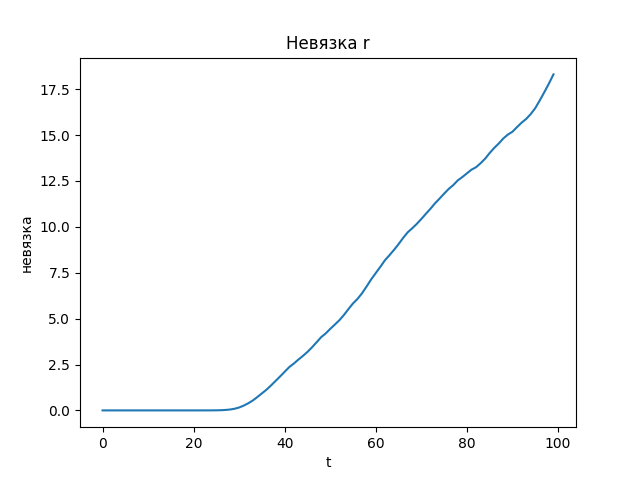
\includegraphics[scale=0.6]{r_div10}
\end{center}
\end{minipage}
\begin{minipage}{0.47\textwidth}
\begin{center}
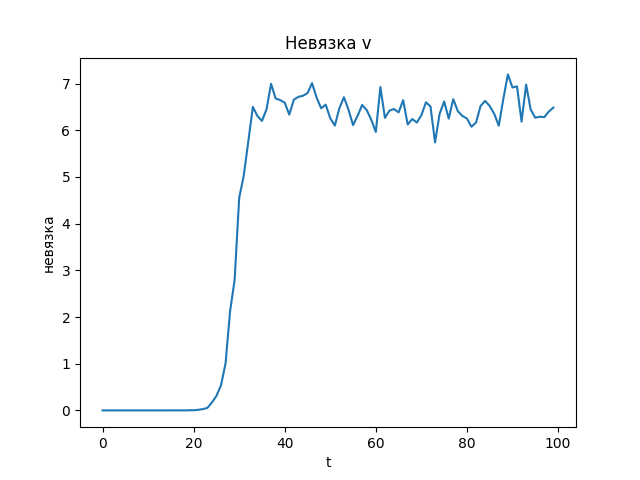
\includegraphics[scale=0.6]{v_div10}
\end{center}
\end{minipage}
\[\textit{Невязки при ratio = 10}\]\\
Система с 216 частицами и $dt_0$ = 0.001 были инициализированы при помощи кода с семинара. При трех параметрах ratio = 2, 5, 10 было оценено время выхода невязки v на плато: 35, 34 и 33 временных интервала соответсвенно.
Так как динамическое время памяти является пределом "значений выхода невязки v на плато", можно сделать вывод, что время динамической памяти системы $\approx$ 30 временным интервалам $t_{dm} = 2.9 \pm 0.5$.

Также можем убедиться, что это правда распределение Максвелла, линеаризовав график N(v) и построив зависимость $ln(\frac{N}{v^2}) (v^2)$:
\begin{center}
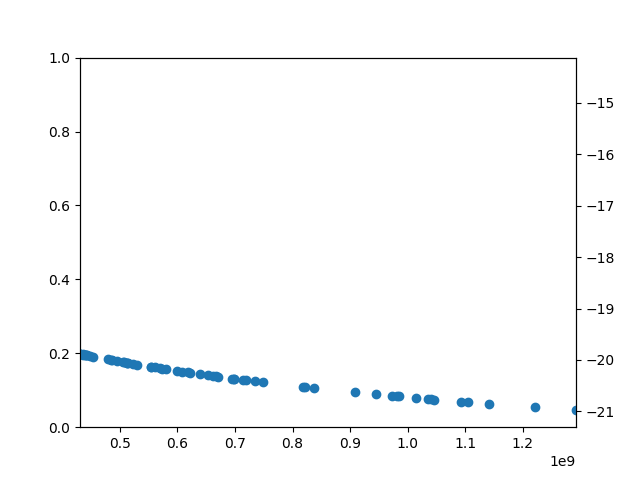
\includegraphics[scale=0.8]{max}
\end{center}
\[\textit{Линеаризация Максвелла}\]

\part{Уравнение состояния}
\section{Зависимость давления и сжимаемости системы от плотности}
\begin{minipage}{0.47\textwidth}
\begin{center}
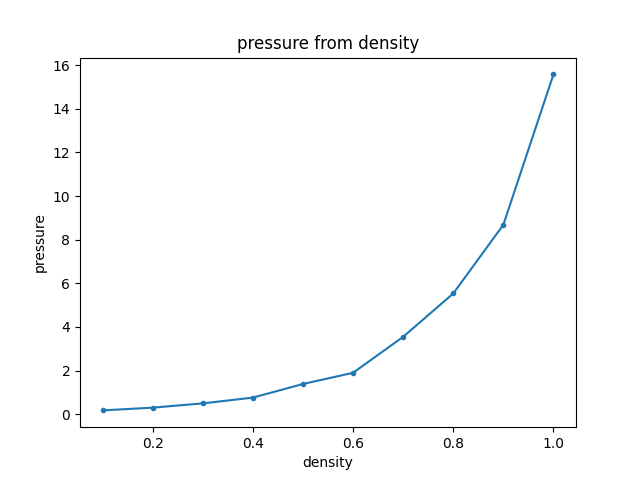
\includegraphics[scale=0.6]{pressure}
\end{center}
\[\textit{Зависимость давления от плотности}\]
\end{minipage}
\begin{minipage}{0.47\textwidth}
\begin{center}
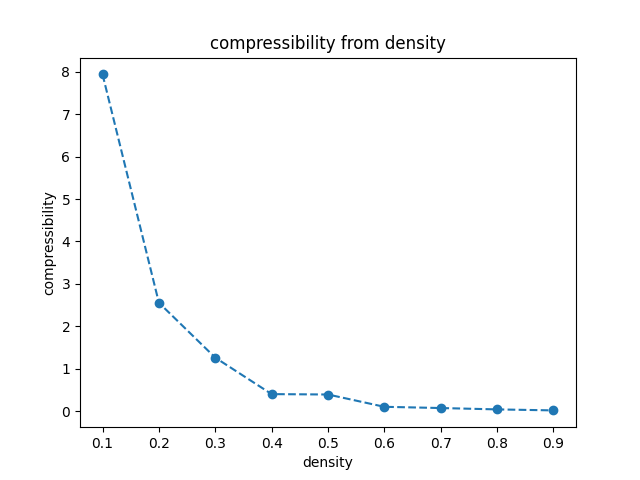
\includegraphics[scale=0.6]{comp}
\end{center}
\[\textit{Зависимость сжимаемости от плотности}\]
\end{minipage}\\\\
Измерения проводились в системе с 216 частицами с поддерживаемой термостатом тепературой T = 2.0. Полученные значения неплохо согласуются с табличными. Сжимаемость была посчитана по формуле:
\[\beta = -\frac{1}{V}\frac{dV}{dp} = \frac{1}{\rho}\frac{d\rho}{dp}\]

\section{Отношение давлений}
\begin{center}
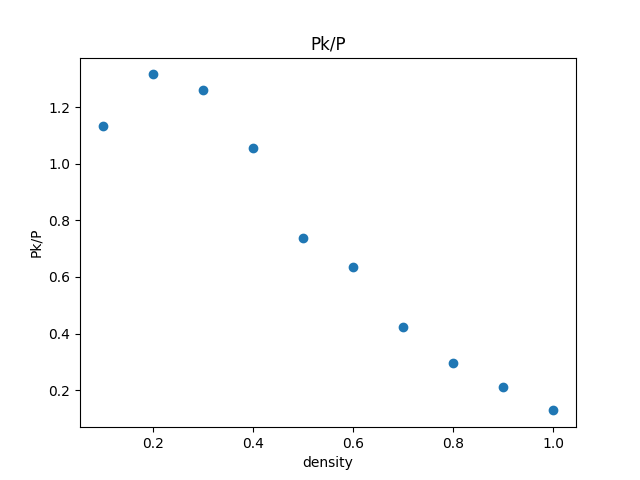
\includegraphics[scale=0.6]{pk}
\end{center}
\[\frac{P_k}{P_k - P_{vir}} \textit{ от плотности}\]
Из графика видно, что $P_k / P$ убывает с ростом плотности.

\section{Формула поправки давления}
\begin{center}
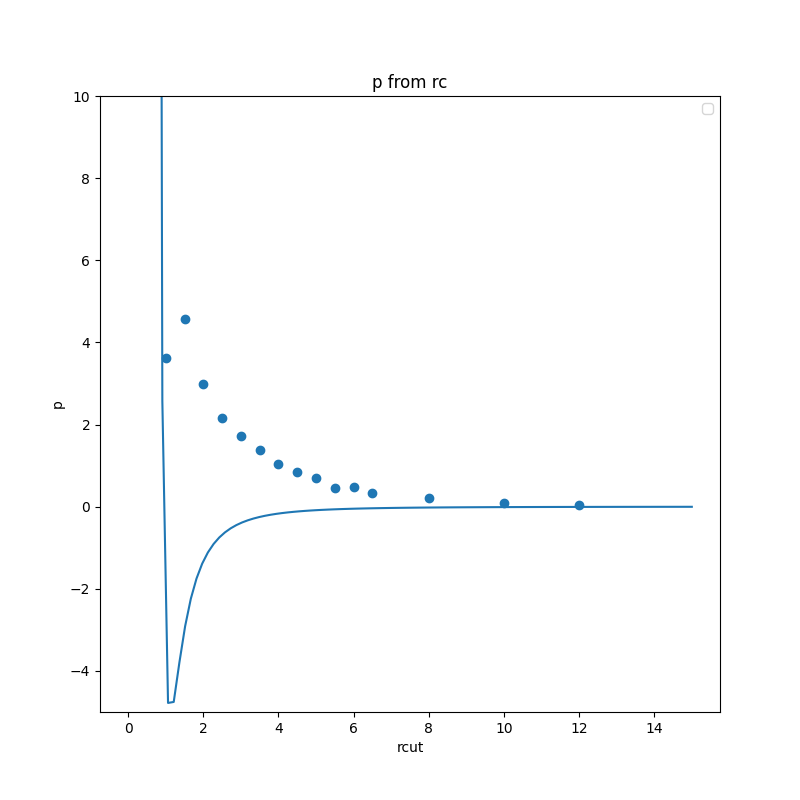
\includegraphics[scale=0.8]{pcor}
\end{center}
\[\textit{Точками на графике обозначена разность давлений с обрезкой и без обрезки,}\]
\[\textit{а кривой - теоретическая зависимость поправки от }r_cut\]

Измерения проводились в системе с 216 частицами при T = 2.0 b dt = 0.001. Давление без обрезки $P_0 = 1.387$. В районе двойки-единицы, думаю, точки уходят вверх (вопреки зависимости), потому что частицы без сопротивления приближаются в зону других частиц, где на них начинает действовать значительная сила, разгоняя, но при отдалении уже не притягивая. Поэтому кинетический вклад в давление растет, а вириальная составляющая уменьшается. Начиная примерно с $r_{cut} = $ 8 $\Delta p \rightarrow 0$.

\part{Оценка ошибки усреднения}
Измерения получены для 216 частиц с dt = 0.001 в 100000 шагов. Методом блочных средних для полной энергии системы было получено:
\begin{center}
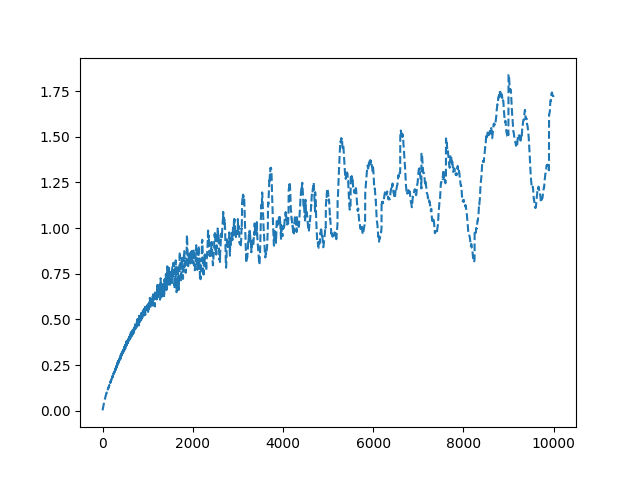
\includegraphics[scale=0.8]{err}
\end{center}
\[\textit{График метода блочных средних}\]
\begin{center}
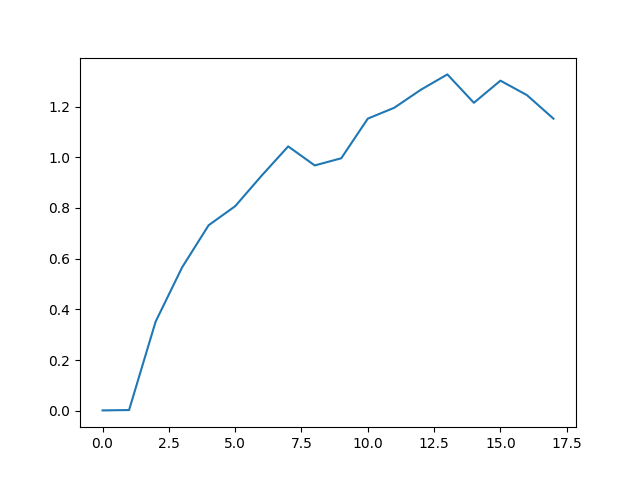
\includegraphics[scale=0.8]{err2}
\end{center}
\[\textit{График метода блочных средних с шагом в 500}\]
\begin{center}
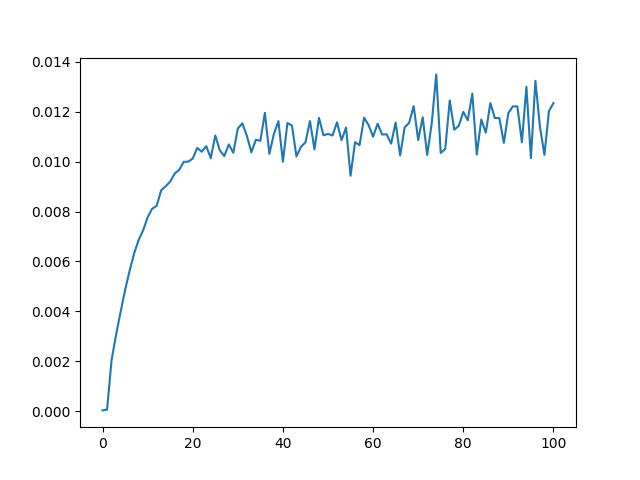
\includegraphics[scale=0.8]{fig}
\end{center}
\[\textit{График метода блочных средних с 1000000 точек}\]

То есть выходит на плато примерно при размере блоков равном 4000. Таким образом $\sigma^2(E) \approx 30$, в то время как полная энергия E = 740. Большая относительная ошибка объяснима маленьким количеством частиц и достаточно большой температурой.

\end{document}